\section{Project Overview}

    Physical infrastructure is a large and complicated subject, encompassing everything from running water to mains electricity. Below I have listed the main features included in physical infrastructure:

    \begin{itemize}
        \item \textbf{Transportation:} Road and highway networks; Mass transit systems; Railways; Canals; Seaports; Airports; Bicycle paths / pedestrian walkways

        \item \textbf{Energy:} Electrical power network; Natural gas pipelines; Petroleum pipelines; Coal production and processing

        \item \textbf{Water management:} Drinking water supply; Sewage collection; Drainage systems; Irrigation systems; Flood control systems; Coastal management

        \item \textbf{Communications:} Postal service; Telephone networks; Mobile phone networks; Television and radio stations; Internet services; Communications satellites; Undersea cables

        \item \textbf{Solid waste management:} Landfills; Incinerators; Hazardous waste disposal
    \end{itemize}

    Computer modelling systems could be developed for any one of these areas, allowing users to prototype infrastructure designs before the costly process of constructing it. For this project I have chosen to focus on the Transportation sector, as it can include some of the most expensive forms of infrastructure.

    Naturally the major responsibility of transportation infrastructure goes towards the construction and maintenance of road networks, including but not limited to junctions, roundabouts, highways and traffic lights.
    These networks can get very complicated and difficult to manage, for example the UK's so called "Spaghetti junction" in Birmingham.

    \begin{figure}[h]
        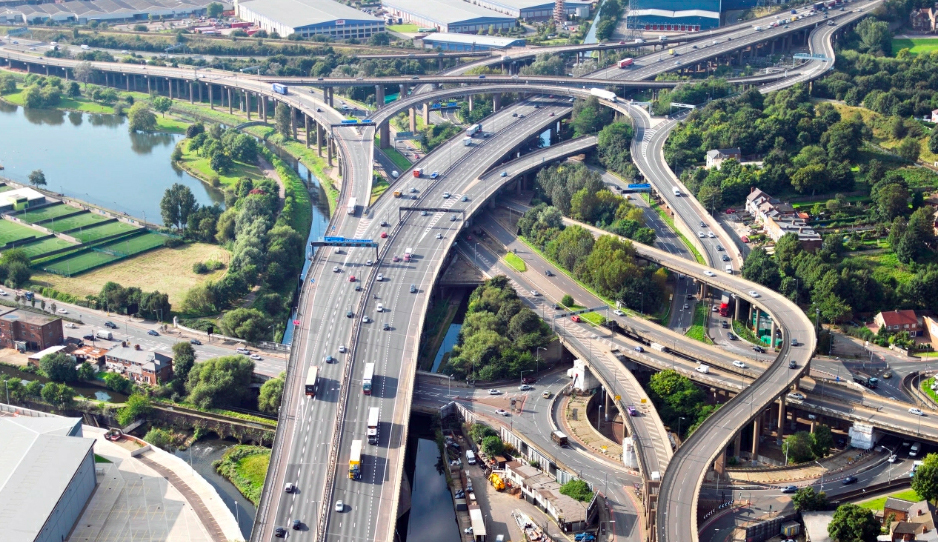
\includegraphics[width=0.5\textwidth]{Spaghetti-Junction.jpg}
        \centering
        \caption{Birmingham's "Spaghetti junction" \cite{Spaghetti-Junction}}
    \end{figure}

\newpage

\section{The Problem}

    Development of transportation infrastructure is a very expensive and time consuming process that comes with many challenges. First is the issue of safety, most road traffic accidents occur at low speeds. Many planning stages are required to ensure the build meets the required standards even before construction begins, taking a lot of time and manpower. Secondly, road networks be made reliable and maintainable, future development and expansion must be considered with roads designed to handle future predicted traffic patterns. Finally, roads need to be considered for financial viability, it is much cheaper to build the right road once than to keep fixing the wrong road.

\section{Current Systems}

    \subsection{AnyLogic - Road Traffic Simulation Software}

        AnyLogic - Road Traffic Simulation Software \cite{AnyLogic} is an industry-level program used for analysing traffic patterns and behaviours, below are a couple images of the program. I chose this program as it would be beneficial to analyse a commercial grade example in order to inform my own project.

        \begin{figure}[ht]
            \centering
            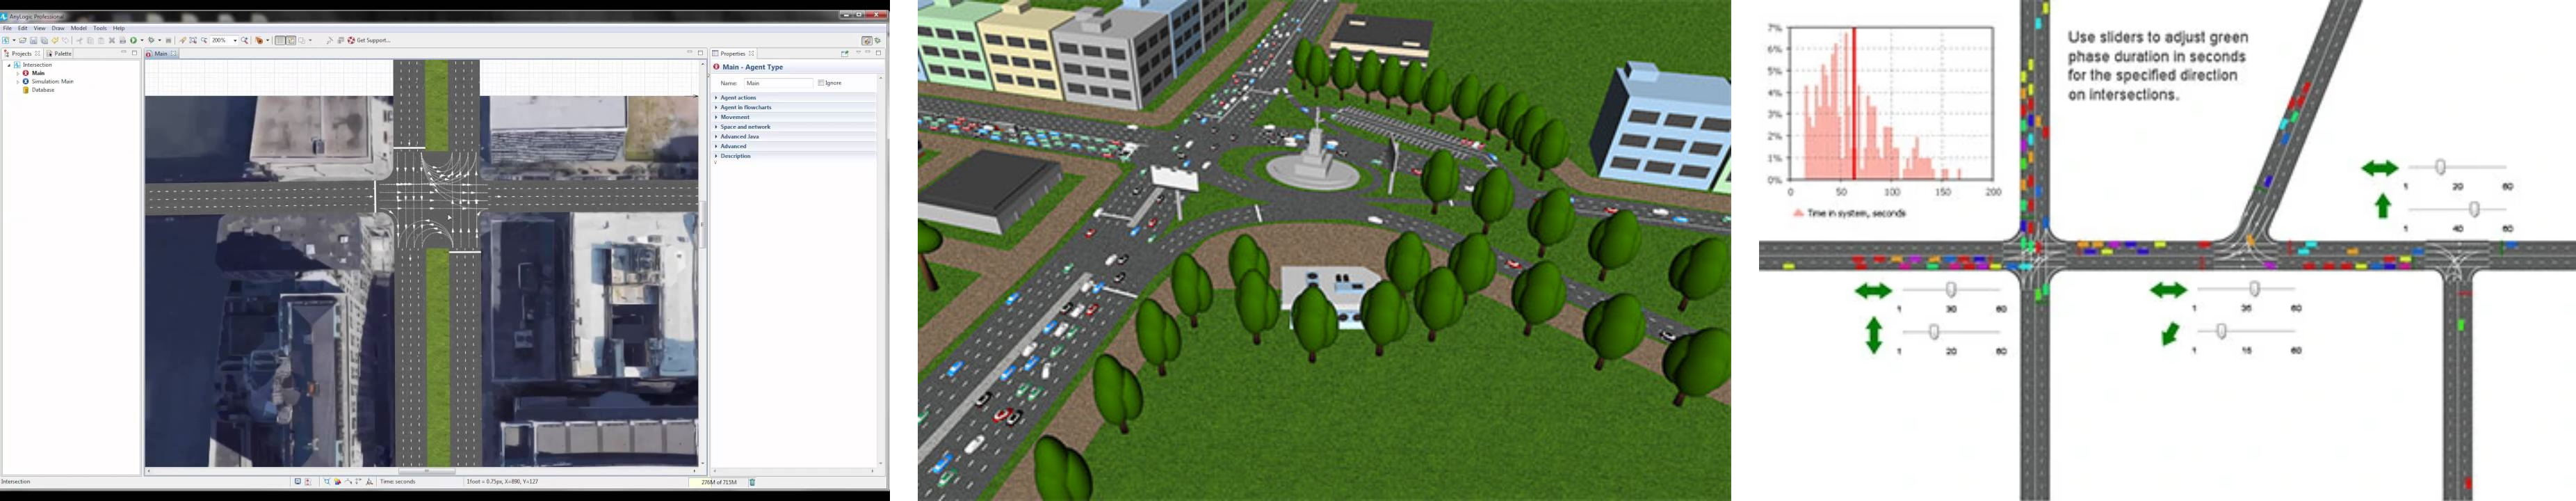
\includegraphics[width=0.9\textwidth]{anylogic-images.jpg}
            \caption{Screenshots from AnyLogic road traffic simulation software}
        \end{figure}

        \prosandcons{
            \item Sophisticated and accurate Simulation.
            \begin{itemize}
                \item This program simulates vehicles in 3D using a physics engine, this allows the simulation to be as "true to life" as possible as well as simulating vehicle collisions.
                \item The model allows for many road features such as traffic lights, roundabouts and speed limits; along with many more.
            \end{itemize}
            \item Comprehensive range of tests.
            \begin{itemize}
                \item The simulation allows the user to test the network under many different situations such as differences in traffic, vehicle size or weather conditions.
                \item This program can also display information and provide warnings of extreme road curvatures, alerting the user if the road is too sharp for vehicles travelling at a given speed.
            \end{itemize}
            \item Graphical data output
            \begin{itemize}
                \item After a simulation has been performed the program produces a range of graphs to show the data collected, these can be customised and exported as well as files containing the raw data collected.
            \end{itemize}
        }{
            \item 3D road network visualisation.
            \begin{itemize}
                \item While the 3D interface for the road network allows for a more grounded representation in the real-world it also detracts from the focus on the road network itself and can make it more difficult to understand it's complexities.
            \end{itemize}
            \item Unintuitive interface.
            \begin{itemize}
                \item Largely as a result of the enormous number of features contained in this software, the interface has become clunky and unintuitive. Along with the lack of tutorials or comprehensive help menus, this drastically reduces the accessibility of the product to new users.
            \end{itemize}
        }

    \subsection{Mini Motorways}

    \begin{quote}
        "Mini Motorways is a game about drawing the roads that drive a growing city. Build a road network, one road at a time, to create a bustling metropolis. Redesign your city to keep the traffic flowing, and carefully manage upgrades to meet the changing demands."\cite{mini-motorways}
    \end{quote}

    Unlike the first example, this is not an industry-level program, instead it is a video game however there were a few reasons I still thought it useful to explore this program. Firstly in my experience testing the game I found the road building system to be incredibly intuitive and user-friendly, as well as finding the art style very inobtrusive to the gameplay.

    \begin{figure}[ht]
        \centering
        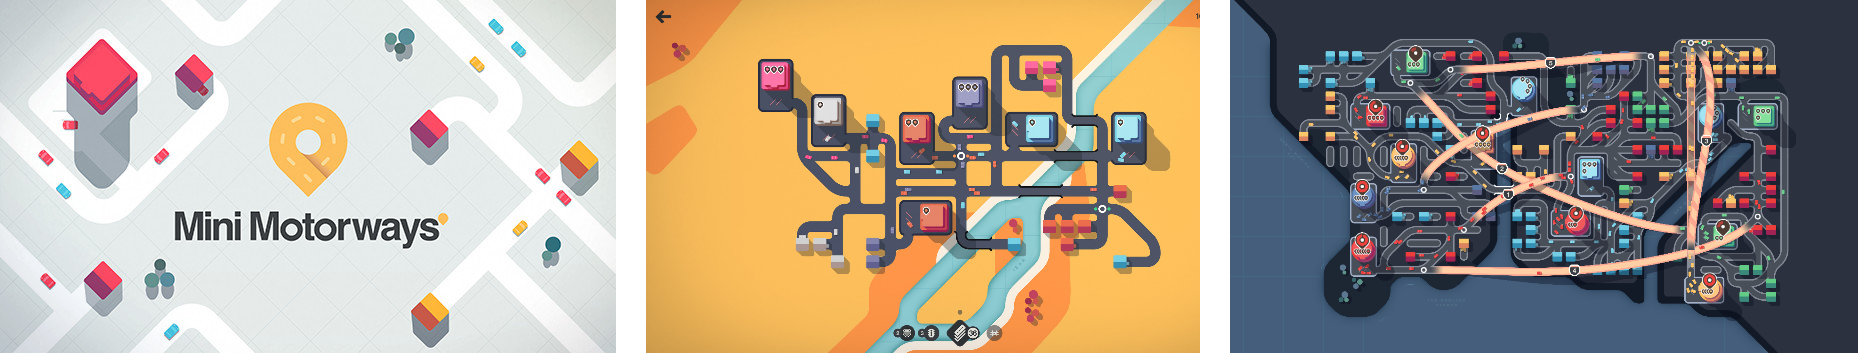
\includegraphics[width=0.9\textwidth]{mini-motorways-images.jpg}
        \caption{Screenshots from Mini Motorways}
    \end{figure}

    \prosandcons{
        \item Intuitive road building system.
        \begin{itemize}
            \item The simple click and drag system for building road, along with a series of well established hotkeys and visual key press responses, make this system very intuitive and friendly for new users.
            \item Despite the very accessible interface the game contains a very short tutorial section that teaches the basics of the control scheme, ensuring that every user can use it effectively.
        \end{itemize}
    }{
        \item
    }

    \subsection{Eclipse SUMO}

\section{End user}

    The intended user of for this project would be someone in a position of urban development or planning. For this project I got in touch with \textbf{[insert contact here, still waiting on a reply]}. Below is a transcript of the interview I conducted with them:

\section{Research}

    \subsection{Traffic laws}

        This project will be based off the UK Highway Code \cite{Highway-Code} as of the latest update (23 March 2021). This document contains all laws and regulations for driving in the UK. The relevant points include:

        \begin{itemize}
            \item Normal driving position is considered the leftmost lane of the road and should be assumed whenever possible
            \item Right-of-way is given to the major road when emerging from a junction
            \item When entering a roundabout, you must give way to vehicles on your right
            \item Is it recommended to maintain a two second separation distance from the vehicle in front
        \end{itemize}

        These rules will be used to inform how the vehicles in the simulation operate in different circumstances. Although it may be noted that not all vehicles follow these laws strictly, so deviations may be added to account for this.

    \subsection{Graphs}

        The natural way to represent any kind of network (including road networks) programmatically is using a graph, so I will conduct some preliminary research into this topic.

        Graphs are an abstract data structure used to describe a set of vertices and the edges connecting them, both vertices and edges can have associated values. This is a very useful structure in computer science as it can be used to model a wide range of existing data such as power grids and social networks. Graphs also come with a wide range of existing algorithms for operating on them such as Dijkstra's shortest path algorithm or the A* search algorithm.

        Described below are the two most common data structures used to describe graphs:

        \begin{itemize}
            \item \textbf{Adjacency list} - Vertices are stored as objects containing a list of it's own adjacent vertices.
            \item \textbf{Adjacency matrix} - A two-dimensional matrix where each cell represents the edge (or lack of edge) from the vertex described by the row to the vertex described by the column.
        \end{itemize}

        Each implementation has its advantages and disadvantages \autoref{graph-time-complexities} shows the time complexity of each operation over these two structures.


        \begin{table}[h]
            \centering
            \begin{tabular}{|p{0.2\linewidth}|p{0.2\linewidth}|p{0.2\linewidth}|} \hline
            & Adjacency list & Adjacency matrix \\ \hline
            Store graph   & $O(|V|+|E|)$ & $O(|V|^2)$ \\ \hline
            Add vertex    & $O(1)$ & $O(|V|^2)$ \\ \hline
            Add edge      & $O(1)$ & $O(1)$ \\ \hline
            Remove vertex & $O(|E|)$ & $O(|V|^2)$ \\ \hline
            Remove edge   & $O(|V|)$ & $O(1)$ \\ \hline
            Check for adjacency between two vertices & $O(|V|)$ & $O(1)$ \\ \hline
            \end{tabular}
            \caption{Time complexities of different graph implementations \cite{graph-time-complexities}}
            \label{graph-time-complexities}
        \end{table}

        Since road networks are generally optimised for maximum throughput I will also research the graph maximum flow problem as this may be useful in evaluating the networks. Formally, the maximum flow problem is as follows \cite{citation needed}:

        \begin{itemize}
            \item Let $N = (V,E)$ be a network with $s, t \in V$, where $s$ is the source and $t$ is the sink.
            \item The capacity of an edge is the maximum flow that can pass through it, the capacity from vertex $v$ to vertex $u$ is denoted as $c_{uv}$; and flow on the same edge as $f_{uv}$.
            \item The flow network must satisfy two properties:
            \begin{itemize}
                \item Capacity constraint: The flow of an edge cannot exceed it's capacity. \[\forall (u, v) \in E : f_{uv} \leq c_{uv}\]
                \item Conservation constraint: The flow into a vertex must equal the flow exiting a vertex (the source and sink are exceptions).
                \[\forall v \in V \setminus \{s, t\} : \sum_{u : (u, v) \in E} f_{uv} = \sum_{u : (v, u) \in E} f_{vu}\]
            \end{itemize}
            \item The value of flow is the total amount of flow passing from the source to the sink, given by:
            \[|f| = \sum_{v : (s, v) \in E} f_{sv}\]
        \end{itemize}

        The goal of the maximum flow problem is to route as much flow as possible from the source to the sink under these constraints. Many algorithms to compute $f_\text{max}$ have been found including but not limited to Linear Programming, the Ford-Fulkerson algorithm or the Edmonds-Karp algorithm.

        The maximum flow of a road network could be a good indicator of the theoretical maximum efficiency.

    \subsection{Bezier curves}

        Bezier curves are very popular in computer graphics due to their many useful properties, for this project Bezier curves could be used to model the road connections between vertices of the road network.

        The definitions for linear (line), quadratic (3 points) and cubic (4 points) are as follows:

        \begin{align*}
            B_1(t) &= (1 - t)\mathbf{P_0} + t\mathbf{P_1}\\
            B_2(t) &= (1 - t)^2\mathbf{P_0} + 2(1 - t)t\mathbf{P_1} + t^2\mathbf{P_2}\\
            B_3(t) &= (1 - t)^3\mathbf{P_0} + 3(1 - t)^2t\mathbf{P_1} + 3(1 - t)t^2\mathbf{P_2} + t^3\mathbf{P_3}
        \end{align*}

        Where $t$ is an interpolation value where $0 \leq t \leq 1$, where $t=0$ is the start of the curve and $t=1$ is the end. $P$ is a set of control points that define the curve. A Bezier curve $B_n(t)$ can be formed for any order $n \in \mathbb{N}$. Bezier curves in this form are known as "Bernstein polynomial form" and is one of the easiest ways to work with these curves.

        The properties of a Bezier curve include:
        \begin{itemize}
            \item The curve begins at $P_0$ and ends at $P_n$.
            \item The curve is tangent to the line formed by the first 2 control points, and also the line formed by the last 2.
            \item The curve can be interpolated continuously, meaning an arbitrarily precise point can be acquired.
            \item The curve can be easily differentiated, allowing use of it's tangent and normal vectors.
            \item There is also a method for finding the curvature of a Bezier curve at any point along it's length.
        \end{itemize}

        Differentiating a Bezier curve is as easy as differentiating each coefficient in it's "Bernstein polynomial form" with respect to $t$ as each control point can be considered a constant. Which for a cubic Bezier looks like this.

        \begin{align*}
            B_3(t) &= (1 - t)^3\mathbf{P_0} + 3(1 - t)^2t\mathbf{P_1} + 3(1 - t)t^2\mathbf{P_2} + t^3\mathbf{P_3}\\
            \frac{d}{dt}B_3(t) &= \frac{d}{dt}\left[(1 - t)^3\mathbf{P_0} + 3(1 - t)^2t\mathbf{P_1} + 3(1 - t)t^2\mathbf{P_2} + t^3\mathbf{P_3}\right]\\
            &= \frac{d}{dt}\left[(1 - t)^3\mathbf{P_0}\right] + \frac{d}{dt}\left[3(1 - t)^2t\mathbf{P_1}\right] + \frac{d}{dt}\left[3(1 - t)t^2\mathbf{P_2}\right] + \frac{d}{dt}\left[t^3\mathbf{P_3}\right]\\
            &= \frac{d}{dt}\left[(1 - t)^3\right]\mathbf{P_0} + \frac{d}{dt}\left[3(1 - t)^2t\right]\mathbf{P_1} + \frac{d}{dt}\left[3(1 - t)t^2\right]\mathbf{P_2} + \frac{d}{dt}\left[t^3\right]\mathbf{P_3}\\
            \frac{d}{dt}B_3(t) &= (-3t^2 + 6t - 3)\mathbf{P_0} + (9t^2 - 12t + 3)\mathbf{P_1} + (-9t^2 + 6t)\mathbf{P_2} + (3t^2)\mathbf{P_3}
        \end{align*}

        As shown the derivative of a Bezier curve is another linear combination of vectors which can be quickly and easily calculated, returning a vector tangent to the curve at that point. The normal vector can also be derived from this by rotating the tangent vector 90 degrees anti-clockwise.

\section{Proposed Solution}

    My proposed solution consists of a desktop app that allows the user to construct an arbitrary road network and perform tests regarding safety and efficiency, in order to assist in the process of road network development.

\section{Objectives}

    \subsection{Network construction}

    \begin{itemize}
        \item The ability to save and load road networks.
        \begin{itemize}
            \item Graph and road network data should have export functionality to a common file type such as \texttt{.txt} or \texttt{.csv}
            \item The same data should be capable of loading into a separate session of the program, restoring the same network from when it was saved.
        \end{itemize}
        \item
    \end{itemize}

    \subsection{Network testing}
    \begin{itemize}
        \item
    \end{itemize}

    \subsection{Graphical user interface}
    \begin{itemize}
        \item The ability to save and load GUI data along with road network data, loading a saved session should return the screen to the same state as it was left off.
    \end{itemize}
